% F090｜convert 原创简明教学示意图
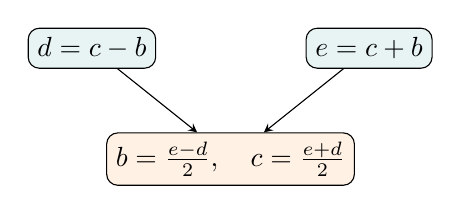
\begin{tikzpicture}[>=stealth,scale=.88]
\node[draw,fill=teal!9,rounded corners] (a) at (0,0){$d=c-b$};
\node[draw,fill=teal!9,rounded corners] (b) at (4,0){$e=c+b$};
\node[draw,fill=orange!10,rounded corners] (c) at (2,-1.6){$b=\frac{e-d}{2},\quad c=\frac{e+d}{2}$};
\draw[->] (a)--(c);\draw[->] (b)--(c);
\end{tikzpicture}
